\documentclass[12pt]{article}
\usepackage[english]{babel}
\usepackage{setspace}
\usepackage[usenames,x11names]{xcolor}
% \usepackage{cmbright}
\usepackage{mathptmx}
\usepackage{amsmath}
\usepackage{amstext}
\usepackage{amsthm}
\usepackage{amssymb}
\usepackage{array}
\usepackage{booktabs}
\usepackage[footnotesize,bf,labelsep=space]{caption}
\usepackage{csquotes}
\usepackage{esvect}
\usepackage{enumitem}
\usepackage{eurosym}
\usepackage{exscale}
\usepackage{fancyhdr}
\usepackage{graphicx}
\usepackage{longtable}
\usepackage{mathrsfs}
\usepackage[version=3]{mhchem}
\usepackage{multirow}
\usepackage{placeins}
\usepackage{rotating}
\usepackage{siunitx}
\usepackage{eurosym}
\usepackage{graphicx}
\usepackage{subcaption}

\usepackage[overlay]{textpos}
\usepackage[colorinlistoftodos,prependcaption,textsize=tiny]{todonotes}
\usepackage{wrapfig}
\usepackage{color, colortbl} 
% \usepackage[colorlinks,allcolors=black]{hyperref}
\usepackage{afterpage}
\usepackage{upgreek}
\usepackage{ulem}
\usepackage[hang,flushmargin]{footmisc}

\usepackage{bibentry}
\bibliographystyle{alpha}
\nobibliography*

  

\usepackage[yyyymmdd]{datetime}
\renewcommand{\dateseparator}{-}

\renewcommand{\baselinestretch}{1.0}

\usepackage{tikz}
\usepackage{pgfplots}
\usepackage{pgfplotstable}
\usepackage{filecontents}
\usepackage[ruled,vlined]{algorithm2e}
\usepackage{varwidth}
\usepackage{adjustbox}
\usetikzlibrary{patterns.meta}
\usepackage{pgfgantt}

\usetikzlibrary{calc}
\tikzset{math3d/.style={z={(-0.65cm,-0.30cm)},y={(0cm,1cm)},x={(0.9cm,-0.15cm)}}}
\usetikzlibrary{shapes.geometric, arrows, intersections, through}
\usetikzlibrary{decorations.text, decorations.shapes, backgrounds}
\usetikzlibrary{arrows.meta}
\usetikzlibrary{colorbrewer}
\usetikzlibrary{patterns}
\usepgfplotslibrary{colorbrewer}
\usepgfplotslibrary{colormaps}


\definecolor{color1}{HTML}{B3E2CD}
\definecolor{color2}{HTML}{FDCDAC}
\definecolor{color3}{HTML}{CBD5E8}
\definecolor{color4}{HTML}{F4CAE4}
\definecolor{color5}{HTML}{E6F5C9}


\newcommand\pgfmathsinandcos[3]{%
  \pgfmathsetmacro#1{sin(#3)}%
  \pgfmathsetmacro#2{cos(#3)}%
}
\newcommand\LongitudePlane[3][current plane]{%
  \pgfmathsinandcos\sinEl\cosEl{#2} % elevation
  \pgfmathsinandcos\sint\cost{#3} % azimuth
  \tikzset{#1/.style={cm={\cost,\sint*\sinEl,0,\cosEl,(0,0)}}}
}
\newcommand\LatitudePlane[3][current plane]{%
  \pgfmathsinandcos\sinEl\cosEl{#2} % elevation
  \pgfmathsinandcos\sint\cost{#3} % latitude
  \pgfmathsetmacro\yshift{\cosEl*\sint}
  \tikzset{#1/.style={cm={\cost,0,0,\cost*\sinEl,(0,\yshift)}}} %
}
\newcommand\DrawLongitudeCircle[2][1]{
  \LongitudePlane{\angEl}{#2}
  \tikzset{current plane/.prefix style={scale=#1}}
   % angle of "visibility"
  \pgfmathsetmacro\angVis{atan(sin(#2)*cos(\angEl)/sin(\angEl))} %
  \draw[current plane,very thin,solid] (\angVis:1) arc (\angVis:\angVis+180:1);
  \draw[current plane,very thin,dashed] (\angVis-180:1) arc (\angVis-180:\angVis:1);
}%this is fake: for drawing the grid
\newcommand\DrawLongitudeCirclered[2][1]{
  \LongitudePlane{\angEl}{#2}
  \tikzset{current plane/.prefix style={scale=#1}}
   % angle of "visibility"
  \pgfmathsetmacro\angVis{atan(sin(#2)*cos(\angEl)/sin(\angEl))} %
  \draw[current plane] (150:1) arc (150:180:1);
  %\draw[current plane,dashed] (-50:1) arc (-50:-35:1);
}%for drawing the grid
\newcommand\DLongredd[2][1]{
  \LongitudePlane{\angEl}{#2}
  \tikzset{current plane/.prefix style={scale=#1}}
   % angle of "visibility"
  \pgfmathsetmacro\angVis{atan(sin(#2)*cos(\angEl)/sin(\angEl))} %
  \draw[current plane,black,dashed, ultra thick] (150:1) arc (150:180:1);
}
\newcommand\DLatred[2][1]{
  \LatitudePlane{\angEl}{#2}
  \tikzset{current plane/.prefix style={scale=#1}}
  \pgfmathsetmacro\sinVis{sin(#2)/cos(#2)*sin(\angEl)/cos(\angEl)}
  % angle of "visibility"
  \pgfmathsetmacro\angVis{asin(min(1,max(\sinVis,-1)))}
  \draw[current plane,dashed,black,ultra thick] (-50:1) arc (-50:-35:1);

}
\newcommand\fillred[2][1]{
  \LongitudePlane{\angEl}{#2}
  \tikzset{current plane/.prefix style={scale=#1}}
   % angle of "visibility"
  \pgfmathsetmacro\angVis{atan(sin(#2)*cos(\angEl)/sin(\angEl))} %
  \draw[current plane,red,thin] (\angVis:1) arc (\angVis:\angVis+180:1);

}

\newcommand\DrawLatitudeCircle[2][1]{
  \LatitudePlane{\angEl}{#2}
  \tikzset{current plane/.prefix style={scale=#1}}
  \pgfmathsetmacro\sinVis{sin(#2)/cos(#2)*sin(\angEl)/cos(\angEl)}
  % angle of "visibility"
  \pgfmathsetmacro\angVis{asin(min(1,max(\sinVis,-1)))}
  \draw[current plane,very thin,solid] (\angVis:1) arc (\angVis:-\angVis-180:1);
  \draw[current plane,very thin,dashed] (180-\angVis:1) arc (180-\angVis:\angVis:1);
}%Defining functions to draw limited latitude circles (for the red mesh)

\newcommand\DrawLatitudeCirclered[2][1]{
  \LatitudePlane{\angEl}{#2}
  \tikzset{current plane/.prefix style={scale=#1}}
  \pgfmathsetmacro\sinVis{sin(#2)/cos(#2)*sin(\angEl)/cos(\angEl)}
  % angle of "visibility"
  \pgfmathsetmacro\angVis{asin(min(1,max(\sinVis,-1)))}
  %\draw[current plane,red,thick] (-\angVis-50:1) arc (-\angVis-50:-\angVis-20:1);
\draw[current plane] (-50:1) arc (-50:-35:1);
}


\newcommand\DrawLatitudeCircleredCoord[4][1]{
  \LatitudePlane{\angEl}{#2}
  \tikzset{current plane/.prefix style={scale=#1}}
  \pgfmathsetmacro\sinVis{sin(#2)/cos(#2)*sin(\angEl)/cos(\angEl)}
  % angle of "visibility"
  \pgfmathsetmacro\angVis{asin(min(1,max(\sinVis,-1)))}
  %\draw[current plane,red,thick] (-\angVis-50:1) arc (-\angVis-50:-\angVis-20:1);
\draw[current plane, thick] (-50:1) coordinate (#3) arc (-50:-35:1) coordinate (#4);
}

\newcommand\DrawLongitudeCircleredCoord[4][1]{
  \LongitudePlane{\angEl}{#2}
  \tikzset{current plane/.prefix style={scale=#1}}
   % angle of "visibility"
  \pgfmathsetmacro\angVis{atan(sin(#2)*cos(\angEl)/sin(\angEl))} %
  \draw[current plane] (150:1) coordinate (#3) arc (150:180:1) coordinate (#4);
  %\draw[current plane,dashed] (-50:1) arc (-50:-35:1);
}%for drawing the grid

\tikzset{%
  >=latex,
  inner sep=0pt,%
  outer sep=2pt,%
  mark coordinate/.style={inner sep=0pt,outer sep=0pt,minimum size=3pt,
    fill=black,circle}%
}



\setcounter{topnumber}{1}
\setcounter{bottomnumber}{0}
\setcounter{totalnumber}{2}
\setcounter{secnumdepth}{2}

\setlength{\skip\footins}{16pt}

% COLUMN TYPES

\newcolumntype{x}{>{\small}c}
\newcolumntype{y}{>{\small}l}
\newcolumntype{z}{>{\small}r}
\newcommand{\tabitem}{~~\llap{\textbullet}~~}

% LENGTH VARIABLES

\newcommand*{\tablewidth}{215mm} \newcommand*{\figurefactor}{0.8}
\newcommand*{\subfigurefactor}{0.425}
\newcommand{\comment}[1]{\textcolor{blue}{(#1)}}

% NUMBERING EQUATIONS AND FIGURES

\renewcommand{\theequation}{\arabic{equation}}
%\renewcommand{\theequation}{\thesection.\arabic{equation}}
%\numberwithin{equation}{section}
\renewcommand{\thefigure}{\arabic{figure}}
%\renewcommand{\thefigure}{\thesection.\arabic{figure}}
%\numberwithin{figure}{section}
\renewcommand{\thetable}{\arabic{table}}
%\renewcommand{\thetable}{\thesection.\arabic{table}}
%\numberwithin{table}{section}
\renewcommand{\thefootnote}{\fnsymbol{footnote}}
\newcommand{\D}{\displaystyle}
\newcommand{\T}{\textstyle}

\renewcommand{\thefootnote}{\arabic{footnote}}

% TEXT LAYOUT (Letter = 216mm x 279mm)
\usepackage[letterpaper]{geometry}
\setlength{\headsep}{0.3cm}
\setlength{\headheight}{1cm}
\geometry{textwidth=176.5mm, textheight=239.5mm}
\renewcommand{\headrulewidth}{0pt}

%% TODO options
\usepackage{xargs}
\newcommandx{\unsure}[2][1=]{\todo[linecolor=red,backgroundcolor=red!25,bordercolor=red,#1]{#2}}
\newcommandx{\change}[2][1=]{\todo[linecolor=blue,backgroundcolor=blue!25,bordercolor=blue,#1]{#2}}
\newcommandx{\info}[2][1=]{\todo[linecolor=OliveGreen,backgroundcolor=OliveGreen!25,bordercolor=OliveGreen,#1]{#2}}
\newcommandx{\improvement}[2][1=]{\todo[linecolor=Plum,backgroundcolor=Plum!25,bordercolor=Plum,#1]{#2}}



\definecolor{darkgreen}{rgb}{0.0, 0.2, 0.13}
\usepackage[framemethod=TikZ]{mdframed}
\newcounter{theo}[section]\setcounter{theo}{0}
\renewcommand{\thetheo}{\arabic{chapter}.\arabic{theo}}

\newcounter{publications}[section]\setcounter{publications}{0}
\renewcommand{\thetheo}{\arabic{chapter}.\arabic{publications}}
\newenvironment{publications}[2][0]{%
    \refstepcounter{publications}
    % Code for box design goes here.
    \ifstrempty{#1}%
    % if condition (without title)
    {\mdfsetup{%
        frametitle={%\ ~
            \tikz[baseline=(current bounding box.east),outer sep=0pt]
            \node[rounded corners=2pt,anchor=east,rectangle,fill=darkgreen!65]
            {\strut \small \ \color{white}{Related publications\ ~}};}
        }%
    % else condition (with title)
    }{\mdfsetup{%
        frametitle={%
            \tikz[baseline=(current bounding box.east),outer sep=0pt]
            \node[rounded corners=2pt,anchor=east,rectangle,fill=darkgreen!65]
            {\strut \small \ \color{white}{Third-party funding:~#1\ ~}};}%
        }%
    }%
    % Both conditions
    \mdfsetup{%
        innertopmargin=0pt,linecolor=darkgreen!65,%
        linewidth=1pt,topline=true,%
        roundcorner=3pt,frametitleaboveskip=\dimexpr-\ht\strutbox\relax%
    }
\begin{mdframed}[backgroundcolor=darkgreen!5]\relax\sloppy\small}{%
\end{mdframed}}

\setlength{\belowcaptionskip}{-10pt}

\newgantttimeslotformat{stardate}{% \def\decomposestardate##1.##2\relax{%
\def\stardateyear{##1}\def\stardateday{##2}% }% \decomposestardate#1\relax%
\pgfcalendardatetojulian{\stardateyear-01-01}{#2}% \advance#2 by-1\relax%
\advance#2 by\stardateday\relax%
}


\newganttlinktype{rdldr*}{%
  \draw [/pgfgantt/link]
    (\xLeft, \yUpper) --
    (\xLeft + \ganttvalueof{link bulge 1} * \ganttvalueof{x unit},
      \yUpper) --
    ($(\xLeft + \ganttvalueof{link bulge 1} * \ganttvalueof{x unit},
      \yUpper)!%
      \ganttvalueof{link mid}!%
      (\xLeft + \ganttvalueof{link bulge 1} * \ganttvalueof{x unit},
      \yLower)$) --
    ($(\xRight - \ganttvalueof{link bulge 2} * \ganttvalueof{x unit},
      \yUpper)!%
      \ganttvalueof{link mid}!%
      (\xRight - \ganttvalueof{link bulge 2} * \ganttvalueof{x unit},
      \yLower)$) --
    (\xRight - \ganttvalueof{link bulge 2} * \ganttvalueof{x unit},
      \yLower) --
    (\xRight, \yLower);%
}
\ganttset{
  link bulge 1/.link=/pgfgantt/link bulge,
  link bulge 2/.link=/pgfgantt/link bulge}
  
\hyphenation{in-com-press-ible}
\hyphenation{com-press-ible}

\newcommand{\link}[3][blue]{\hyperlink{#2}{\color{#1}{#3}}}%

% \numberwithin{page}{section}
% \renewcommand{\thepage}{\thesection-\arabic{page}}
\usepackage{titlesec}
\titleformat{\section}{\normalsize\bfseries}{\thesection}{1em}{}


\fancypagestyle{firststyle}
{
   \fancyhf{}
   \fancyfoot[C]{\thepage}
   \renewcommand{\headrulewidth}{0pt} % removes horizontal header line
}
\fancyhead[l]{}
\fancyhead[r]{Internship project description: \textbf{Intern} \hfill Written by: \textbf{PhD Candidate}}
\setlength{\parindent}{10pt}

\DeclareTextFontCommand{\emph}{\it}

\makeatletter
\renewcommand{\fnum@figure}{Fig.~\thefigure}
\makeatother
\newcommand\Dganttbar[4]{%
  \ganttbar{#1}{#3}{#4}\ganttbar[inline,bar label font=\footnotesize]{#2}{#3}{#4}
}


\makeatletter
\DeclareRobustCommand\em
  {\@nomath\em \ifdim \fontdimen\@ne\font >\z@
     \eminnershape \else \slshape \fi}%
\makeatother



\usepackage{array}
\newcommand{\PreserveBackslash}[1]{\let\temp=\\#1\let\\=\temp}
\newcolumntype{C}[1]{>{\PreserveBackslash\centering}p{#1}}
\newcolumntype{R}[1]{>{\PreserveBackslash\raggedleft}p{#1}}
\newcolumntype{L}[1]{>{\PreserveBackslash\raggedright}p{#1}}

\begin{document}
\pagestyle{fancy}

\section{Context}
Laser powder bed fusion (LPBF) is a additive manufactoring (AM) process in which thin layers (20-500 $\mu m$) of 
metal powder are spreaded/layered onto a build plate. Inbetween each deposited layers, the metal particles
are being selectively melted using a laser. As a result, the individual particles fuse together and with the 
underneath powder layers. 
This layer-by-layer process is repeted thousands of time depending on the size of the part being made. 
\\

\noindent Like many AM processes, LPBF offers several advantages like freedom in design, 
better performance of fabricated parts, opportunities for massive lightweighting, 
possible cost savings due to reduced part count, on-demand manufacturing, reductions 
of material waste and energy consumption, etc. Despite these promising capabilities, 
the broad adoption of this technology in the industry is still prevented by technical challenges, 
particularly concerning the powder spreading and melting steps.
\\

\noindent This project, in collaboration with the National Research Council (NRC), aims to develop a 
numerical tool to predict and better understand the powder spreading phenomena, 
while other members of the CHAOS lab focus on the laser melting modeling.
\\

\noindent Regarding the importance of powder spreading, many aspects must be considered. This step is 
time-consuming since it can account for up to 25\% of the total manufacturing time. It is also highly 
sensitive to the powder properties such as particle size distribution (PSD), sphericity, cohesivity and 
operating parameters including layer thickness, spreading speed, and blade geometry. A poor 
powder bed, resulting from inadequate spreading, directly affects the quality of the final 
product. Currently, the industry relies on a trial-and-error approach for this step, which is 
not cost-effective. The development of a numerical tool would enhance our understanding of 
of the spreading process at the particle scale, which are not possible to study experimentally. 
This would not only speed up the fabrication process but also improve yields.
\\

\noindent The modeling of the powder spreading step is being carried with Lethe, a high performance open-source 
computational fluid dynamics (CFD), discrete element method (DEM) and coupled CFD-DEM software
based on deal.II, a finite element library. DEM is a time-driven simulation technique based on 
a Lagrangian description of particle motion that predicts the flow of granular matter. Although 
DEM can simulate the powder spreading process, it requires the input of the physical properties (Young modulus, Poisson ratio) 
and contact properties which must be calibrated from experiments (coefficient of restitution, coefficient of sliding friction, 
coefficient of rolling friction, surface energy) of the granular material being model. This internship will focus on the use and 
development of the DEM solver within Lethe, alongside experimental work dedicated to the calibration of these parameters. The main calibration experiment used as part of this experiment will be a granuheap. This experimental devices generates a particle heap in a controlled fashion which can then be used to calibrate friction and cohesive properties of particles (see Figure \ref{fig::raw_heap} and Figure \ref{fig::proc_heap}). 


\begin{figure*}[t!]
  \centering
  \begin{subfigure}[b]{0.45\textwidth}
      \centering
      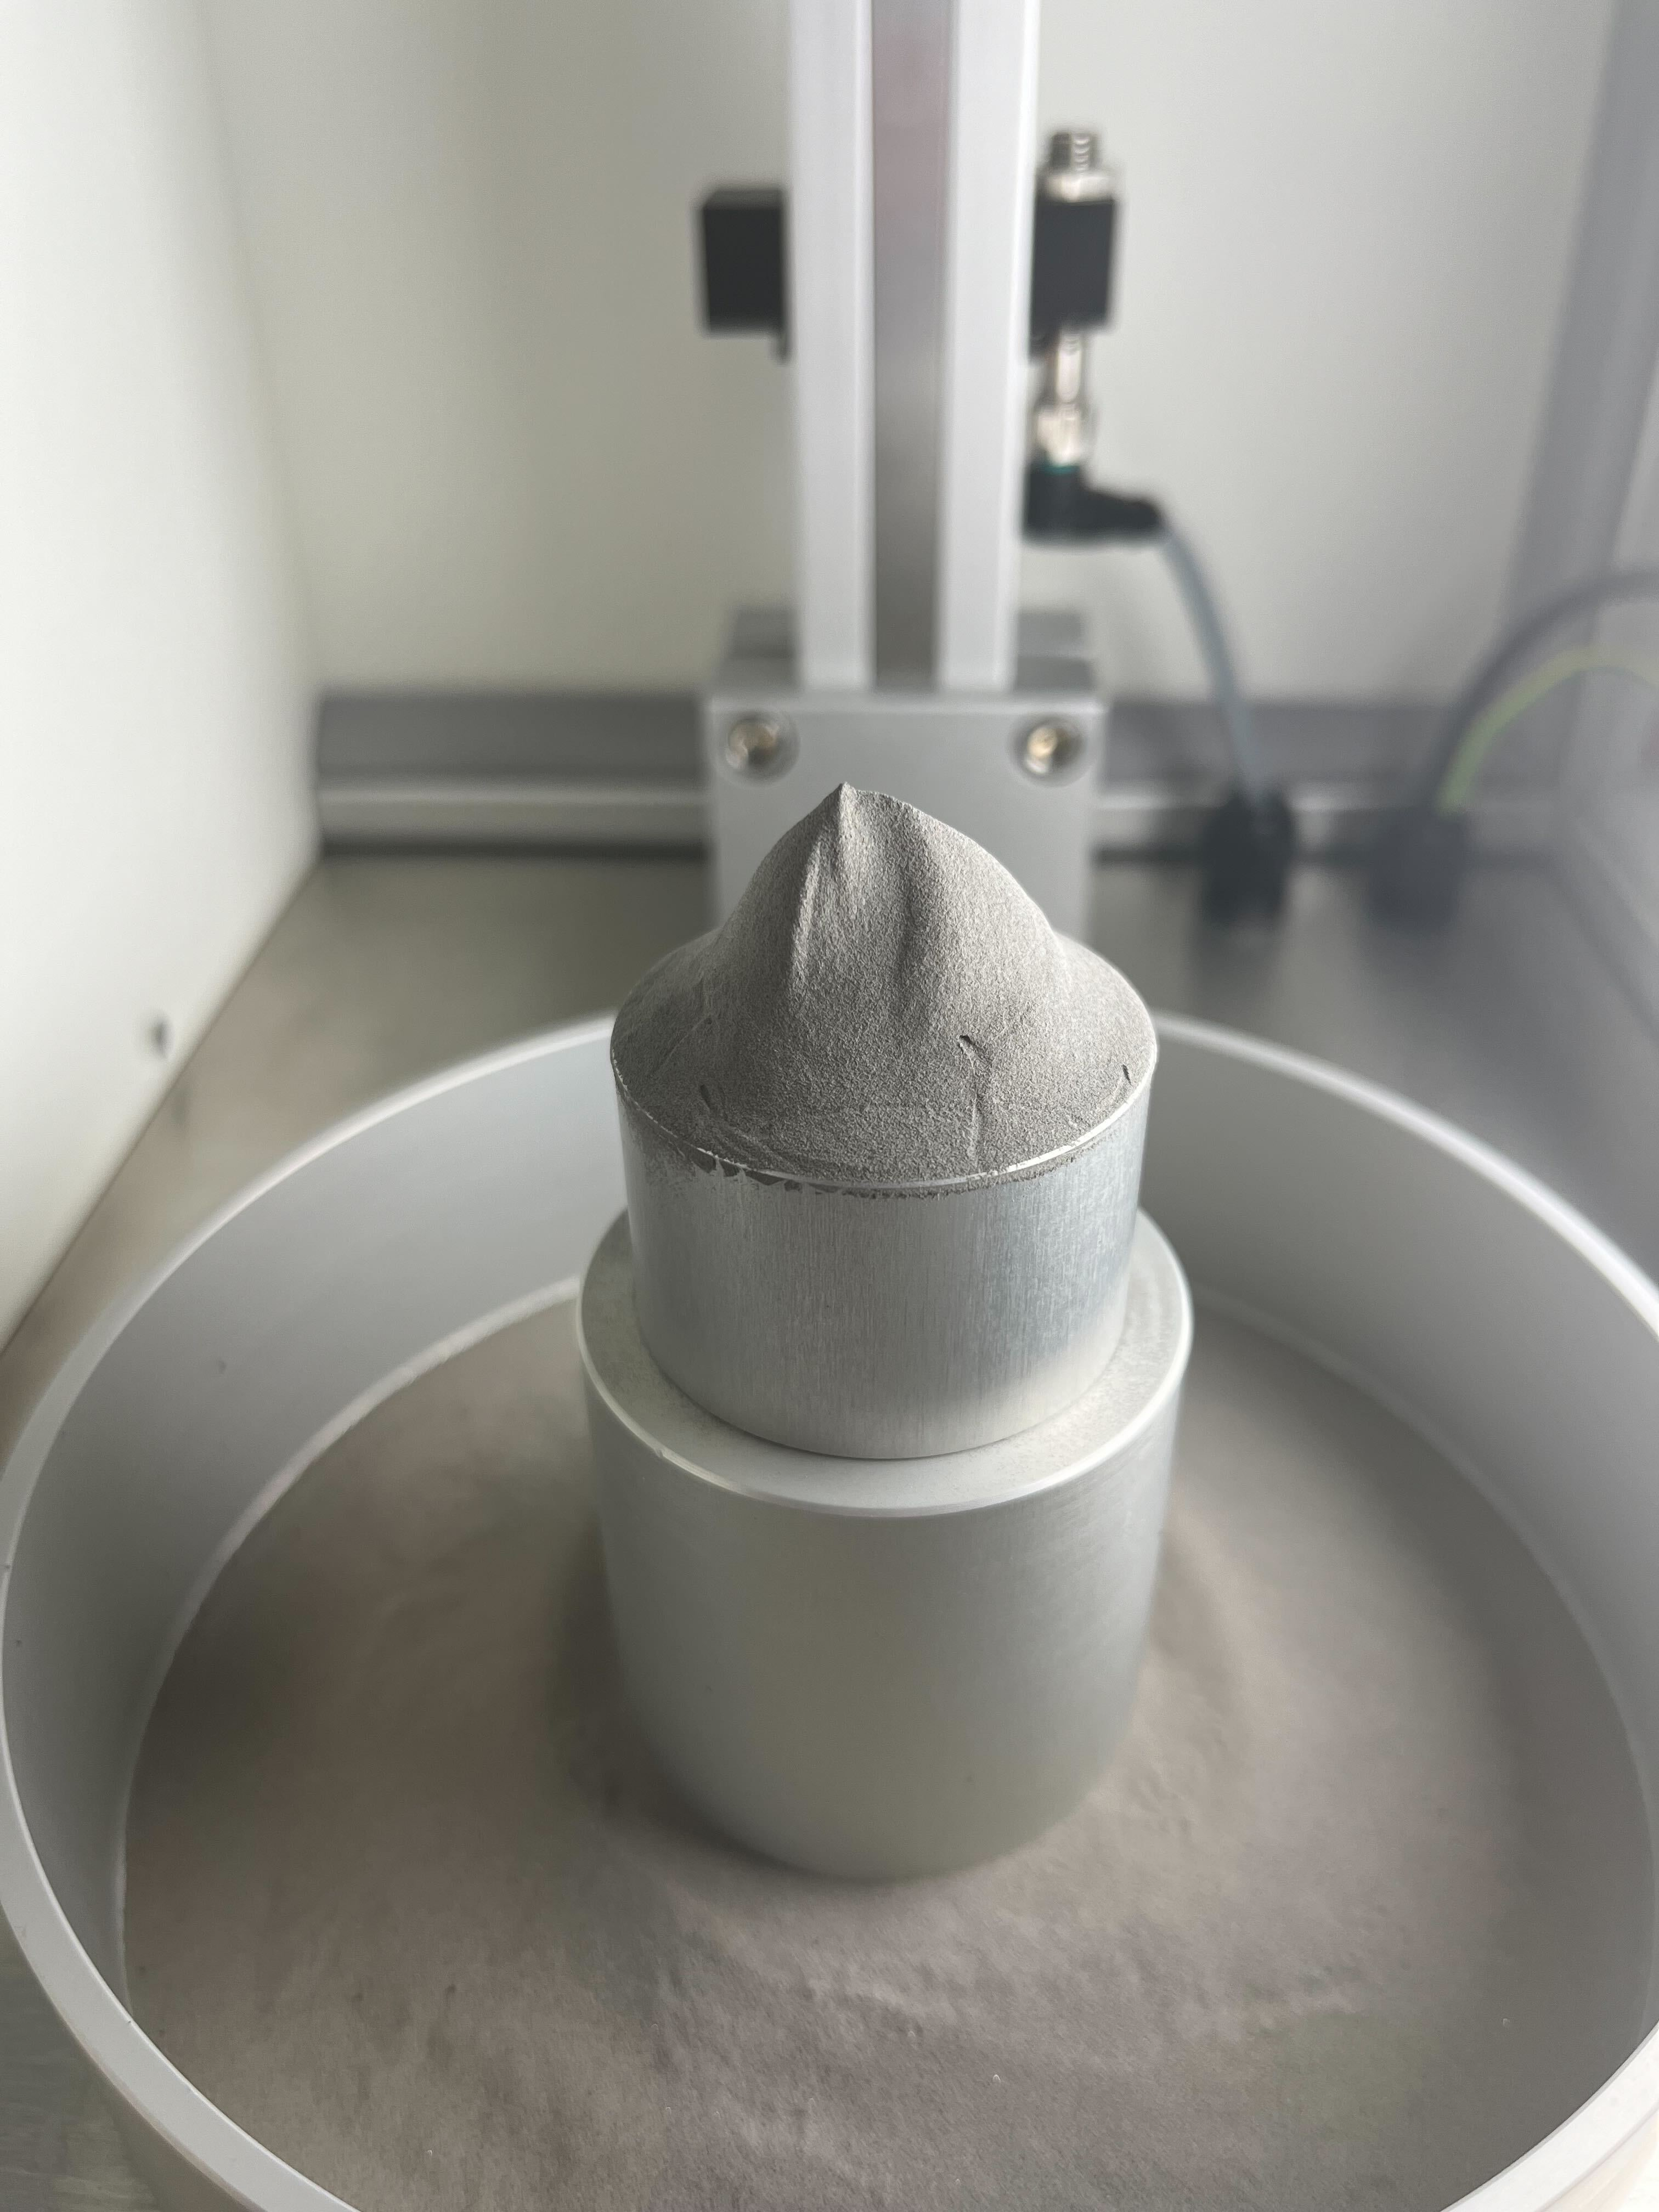
\includegraphics[width=6cm]{images/IMG_4098.jpg}
      \caption{Heap for a cohesive powder} \label{fig::raw_heap}
    \end{subfigure}%
  ~ 
  \begin{subfigure}[b]{0.45\textwidth}
      \centering
      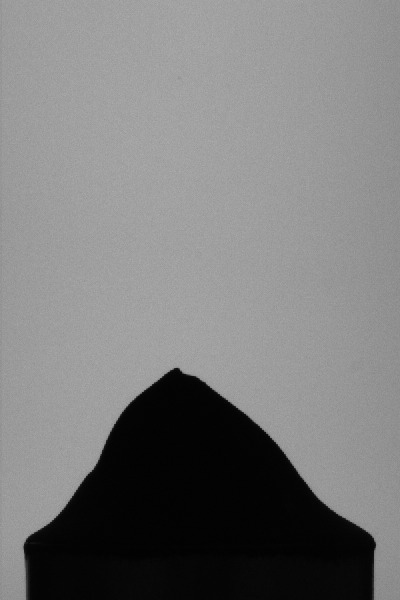
\includegraphics[width=6cm]{images/heap-4.jpg}
      \caption{Image obtained from the heap in the Granuheap} \label{fig::proc_heap}
    \end{subfigure}
  \caption{Illustration of a Granhuheap experiment}
\end{figure*}

\FloatBarrier

\section{Research objectives}

\textbf{General Objective:} 

\begin{enumerate}
  \item Develop the numerical tools to carry the calibration of the DEM model with the Granuheap  (parameter file, image processing and parameter identification).
  \item Calibrate few generic powders using the granuheap.
  \item Develop a post-processing feature for visualizing the force chains in a granular system. 
  \item Create a parametrized Hall flowmeter example with cohesive particles.
\end{enumerate}


\section{Relevant scientific litterature}
\begin{itemize}
  \item \bibentry{meier_modeling_2019}
  \item \bibentry{yao_numerical_2021}
  \item Audrey Collard-Daigneault master's thesis (section 2.1 and 2.2)
\end{itemize}

\newpage
\section{Onboarding documents}

\begin{center}
  \begin{table}[h]
\caption{Resources to learn how to program in C++} 
\centering
\begin{tabular}{p{3cm}|p{8cm}|p{3cm}}
 Topic & References & Section or pages \\
 \hline
 \hline
 A tour of C++ & Stroustrup, B. (2018). A Tour of C++ (2nd ed.). Addison-Wesley. & All \\
 \hline
 Lethe & https://chaos-polymtl.github.io/ & DEM parameter file, examples and theory\\
\end{tabular}
\end{table}
\end{center}


\begin{center}
  \begin{table}[h]
\caption{Resources to learn DEM} 
\centering
\begin{tabular}{p{3cm}|p{8cm}|p{3cm}}
 Topic & References & Section or pages \\
 \hline
 \hline
 Introduction to DEM & Blais et al. \cite{blais2019experimental}&  All \\
 \hline
 Advanced DEM &  Golshan et al. \cite{golshan2023lethe} & All\\
\end{tabular}
\end{table}
\end{center}


\FloatBarrier


\newpage
\section{Gantt Chart}


\begin{figure}[h]

  \begin{ganttchart}[
  group label node/.append style={align=left,text width=11em},
  bar label node/.append style={align=right,text width=11em},
  milestone label node/.append style={align=left,text width=11em},
  Mile1/.style={milestone/.append style={fill=black,align=left,text width=0.6em}},
  x unit=3.2mm,y unit chart=3.8mm,y unit title=4.3mm,vgrid={draw=none,dotted}, title height=1, bar height=.7, group height=0.4,
  ]{0}{31}
    \gantttitle{1-2}{4} 
    \gantttitle{3-4}{4}
    \gantttitle{5-6}{4} 
    \gantttitle{7-8}{4}
    \gantttitle{9-10}{4}
    \gantttitle{11-12}{4}
    \gantttitle{13-14}{4}
    \gantttitle{15-16}{4}\\ 

    \ganttgroup{\footnotesize Onboarding}{0}{3} \\
    \ganttset{bar/.append style={fill=color4}}
    \Dganttbar{\footnotesize SST training}{}{0}{1}\\
    \Dganttbar{\footnotesize Reading}{}{0}{3}\\
    \Dganttbar{\footnotesize Learning how to use Linux}{}{0}{3}\\


    \ganttgroup{\footnotesize  Granu heap example}{4}{11}\\
    \ganttset{bar/.append style={fill=color1}}
   % \Dganttbar{\footnotesize  Labo experiment with Whey}{\scriptsize {}}{4.5}{14}\\ 
   \Dganttbar{\footnotesize Labo experiment with Whey}{}{4}{5}\\
   \Dganttbar{\footnotesize  Parameter file}{\scriptsize {}}{4}{5}\\ 

    \Dganttbar{\footnotesize Map processing \textbf{simulations}}{}{6}{7}\\
    \Dganttbar{\footnotesize Map processing \textbf{experiments}}{}{6}{7}\\
    \Dganttbar{\footnotesize Manual parameter calibration}{}{8}{9}\\
    \ganttbar{\footnotesize Example documentation}{6}{11}\\ 
    \ganttbar{\footnotesize Pull request \& reviews}{10}{11}\\ 

    \ganttmilestone[Mile1]{\footnotesize Lethe example on Granuheap}{11} \\

    \ganttgroup{\footnotesize  Automatic calibration}{12}{23} \\
    \ganttset{bar/.append style={fill=color2}}
    \Dganttbar{\footnotesize Learning NOMAD}{}{12}{13}\\
    \Dganttbar{\footnotesize  Parametrized parameter file}{\scriptsize {}}{12}{15}\\ 

    \Dganttbar{\footnotesize Definition of the cost function}{}{14}{15}\\

    \Dganttbar{\footnotesize First try on example}{}{16}{17}\\
    \Dganttbar{\footnotesize Try on few powders}{}{18}{23}\\
    \Dganttbar{\footnotesize Document \& pull request}{}{14}{23}\\



    \ganttmilestone[Mile1]{\footnotesize Automatic calibratin procedure}{23} \\

    \ganttgroup{\footnotesize Force chain}{0}{0} \\
    \ganttset{bar/.append style={fill=color3}}
    \Dganttbar{\footnotesize Identify algorithm}{}{0}{0}\\
    \Dganttbar{\footnotesize Pseudocode}{}{0}{0}\\
    \Dganttbar{\footnotesize Implementation}{}{0}{0}\\
    \Dganttbar{\footnotesize Pull-request and review}{}{0}{0}\\
    \ganttmilestone[Mile1]{\footnotesize Force-chain visualization}{0} \\

    \ganttgroup{\footnotesize Hall flow with extension}{17}{27} \\
    \ganttset{bar/.append style={fill=color3}}
    \Dganttbar{\footnotesize Geometry + parameter file}{}{17}{21}\\
    \Dganttbar{\footnotesize Pull request andreview}{}{21}{23}\\
    \Dganttbar{\footnotesize Cohesion + neck length}{}{21}{27}\\

    \ganttmilestone[Mile1]{\footnotesize Example + small report}{27} \\


    \ganttlink[link/.style={-stealth,semithick,densely dashed}, link type=rdldr*,link bulge 1=0.5, link bulge 2=0.5,link mid=.937]{elem5}{elem7}
    \ganttlink[link/.style={-stealth,semithick,densely dashed}, link type=rdldr*,link bulge 1=0.5, link bulge 2=0.5,link mid=.937]{elem13}{elem17}
    \ganttlink[link/.style={-stealth,semithick,densely dashed}, link type=rdldr*,link bulge 1=0.5, link bulge 2=0.5,link mid=.937]{elem15}{elem17}
    \ganttlink[link/.style={-stealth,semithick,densely dashed}, link type=rdldr*,link bulge 1=0.5, link bulge 2=0.5,link mid=.937]{elem13}{elem21}
    \ganttlink[link/.style={-stealth,semithick,densely dashed}, link type=rdldr*,link bulge 1=0.5, link bulge 2=0.5,link mid=.937]{elem15}{elem21}
    %\ganttlink[link/.style={-stealth,semithick,densely dashed}, link type=rdldr*,link bulge 1=0.5, link bulge 2=0.5,link mid=.937]{elem21}{elem14}
  %\%ganttlink[link/.style={-stealth,thick,densely dotted}, link type=rdldr*,link bulge 1=0.5, link bulge 2=0.5,link mid=.95]{elem21}{elem14}
  \end{ganttchart}
  \caption{\setstretch{0.95}Work plan of the internship
    \vspace{-0.7em}}
    \label{fig:gantt}
    \end{figure}

\FloatBarrier

\section{Workplace conduct}

\begin{itemize}
  \item \textbf{Number of working hours per week - 35: } The number of working hours are given as an indication. The idea here is to provide you with guidance on the amount of work that is expected.
  \item \textbf{Core working hours - 9:00/15:00: } Core working hours are the hours within the day that the
  intern should be present for meetings and/or discussion with the supervisor and colleagues. 
  \item \textbf{Mandatory meetings: } Every Friday at 1PM. A slide showing the weekly advancements must be filled in beforehand. 
\end{itemize}



%\begin{center}
%  \begin{table}[h]
%\caption{Budget of the internship} \label{budget}

%\centering
%\begin{tabular}{c|R{4.2em}R{4.2em}|R{4.5em}}
% Item & \centering Estimated amount & \centering Unit cost   & \multicolumn{1}{c}{Total} \\
% \hline
% Item 1 & \$ $1\,500$\phantom{)} & \$ 1 & \$ $1\,500$\phantom{)}\\
% Item 2 & \$ $2\,500$\phantom{)} & \$ 1 & \$ $2\,500$\phantom{)}\\
% Item 3 & \$ $3\,500$\phantom{)} & \$ 1 & \$ $3\,500$\phantom{)}\\
% Item 4 & \$ $4\,500$\phantom{)} & \$ 1 & \$ $4\,500$\phantom{)}\\
% \hline
%Total  & - & - &$11\,500$\phantom{)}
%\end{tabular}
%\end{table}
%\end{center}

\section{References}


\bibliography{references.bib}


\end{document}